% Chapter 5: Code generation using patterns

\chapter{Code generation using patterns}

\label{ch:fifth} % For referencing the chapter elsewhere, use \autoref{ch:name} 

\from{PACT begin}
\section{Abstract (PACT)}
Computing systems have become increasingly complex and difficult to program with the emergence of heterogeneous hardware.
Heterogeneity is seen as the answer to the energy-efficiency crisis and as such cannot be avoided.
It is now common to see combinations of multicore CPUs and GPUs (Graphic Processing Units) used in a wide range of systems.
These parallel systems exhibit tremendous computational power at the cost of extreme programming difficulties.

High-level programming languages have been proposed to address this issue.
However, they often rely on complex analysis in the compiler and device-specific implementations to achieve maximum performance.
As a result, compilers and software implementations need to be re-tuned for every device.

In this paper, we propose a novel approach based on algorithmic pattern composition coupled with a powerful, yet simple, set of rewrite rules.
The rules are used to automatically explore algorithmic choices and lower algorithmic patterns into a form amenable to high performance OpenCL code generation.
This approach generates code matching the performance of highly tuned implementations on CPUs and GPUs.
For instance, we match the performance of the level 1\&2 BLAS routines from CUBLAS on Nvidia GPU and even outperform by up to 4.5$\times$ on AMD GPU their own clBLAS implementation.
\from{PACT end}

\from{PACT begin}
\section{Motivation (PACT)}
The overview of our approach is presented in Figure~\ref{fig:highlevel}.
The programmer expresses his problem by writing a \emph{high-level expression} composed of \emph{algorithmic patterns}.
Using a rewrite rule system, we automatically lower this high-level expression into a \emph{low-level expression} consisting of \emph{hardware patterns}.
This rewrite stage explores the algorithmic and optimization choices in the high-level expression.
The generated low-level expression is then fed into our code generator that emits an \emph{OpenCL program}.
This program is finally compiled to machine code by the vendor provided OpenCL compiler.

The biggest advantage of our approach is that there is no analysis or optimizations performed in the code generator.
All optimization decisions are automatically made earlier on in the rule rewriting system.
This results in a clear separation of concern between the high-level patterns used by the programmer and the low-level hardware paradigms that enable performance portability.

\begin{figure}[t]
\centering
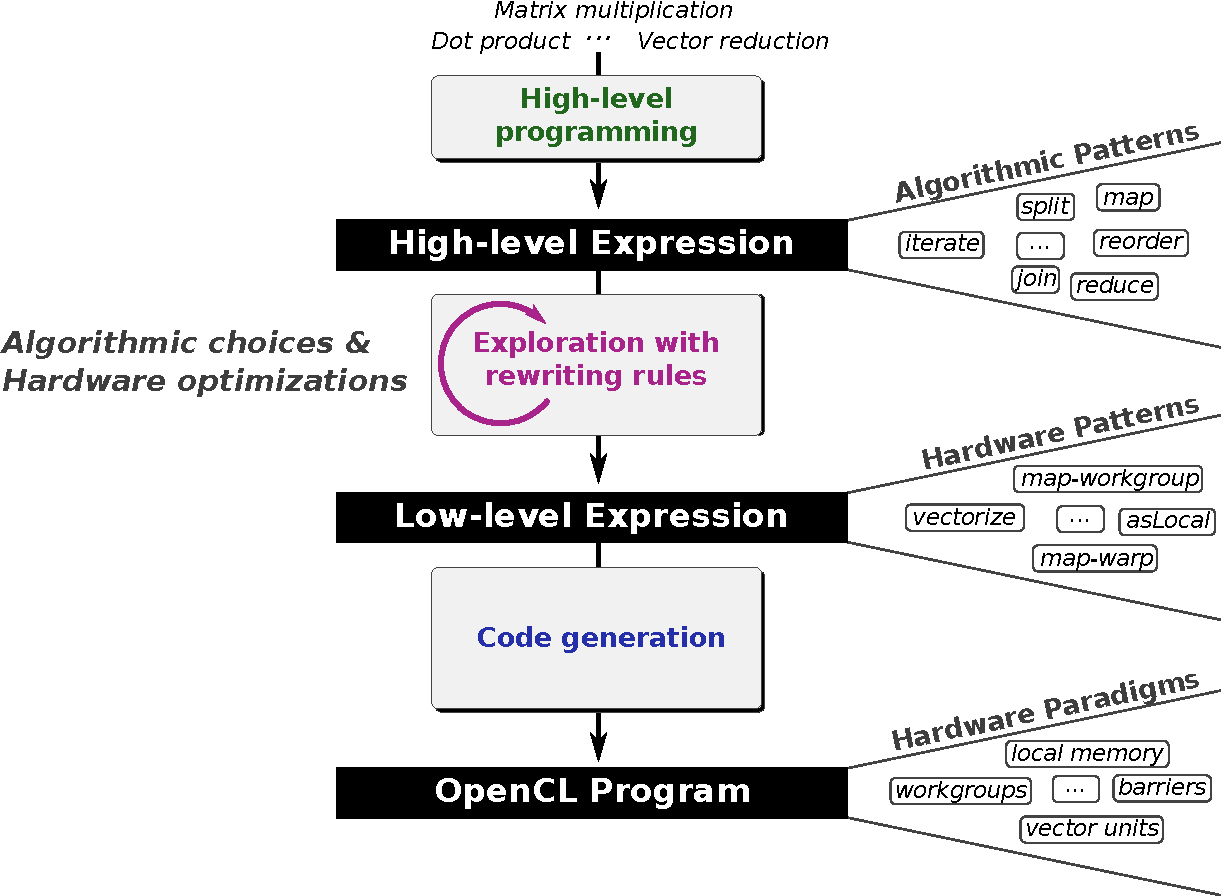
\includegraphics[width=\linewidth]{PACT2014/overview}
\vspace{-15pt}
\caption{
The programmer expresses his problem with high-level algorithmic patterns.
A rule rewriting system explores the space of implementations and lower the high-level expression.
Finally, the code generator produces OpenCL code by mapping the low-level hardware patterns directly to the OpenCL programming model representing the hardware paradigms.}
\label{fig:highlevel}
\end{figure}


\subsection{Example}

\begin{figure}[t]
\centering

\begin{subfigure}[b]{.85\linewidth}
\begin{lstlisting}[mathescape,numbers=left]
def mul3(x) = x * 3    // user-defined function
def vectorMul = map(mul3)        // map pattern
\end{lstlisting}
\caption{\textbf{High-level expression} written by the programmer.}
\label{fig:codeex:map}
\end{subfigure}

\vspace{-5pt}
\begin{minipage}{0.1\linewidth}
\vspace{0pt}
\centering
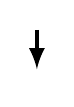
\begin{tikzpicture}[ultra thick]
 \draw [black,   -latex      ] (0,0.5) -- (0,0) node [] {};
\end{tikzpicture}
\end{minipage}
\begin{minipage}{0.25\linewidth}
\vspace{-5pt}
\centering
\textbf{rewrite rules}
\end{minipage}
\begin{minipage}{0.1\linewidth}
\vspace{0pt}
\centering
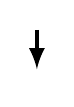
\begin{tikzpicture}[ultra thick]
 \draw [black,   -latex      ] (0,0.5) -- (0,0) node [] {};
\end{tikzpicture}
\end{minipage}

\begin{subfigure}[b]{\linewidth}
\centering
\begin{minipage}{.85\linewidth}
\begin{lstlisting}[mathescape,numbers=left]
def mul3(x) = x * 3
def vectorMul = join $\circ$ map-workgroup(
                  join $\circ$ map-local(
                    vectorize-4(mul3)
                  ) $\circ$ split-4
                ) $\circ$ split-1024
\end{lstlisting}
\end{minipage}
\caption{\textbf{Low-level expression} automatically derived using rewrite rules.}
\label{fig:codeex:impl}
\end{subfigure}

\vspace{-5pt}
\begin{minipage}{0.1\linewidth}
\vspace{0pt}
\centering
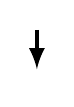
\begin{tikzpicture}[ultra thick]
 \draw [black,   -latex      ] (0,0.5) -- (0,0) node [] {};
\end{tikzpicture}
\end{minipage}
\begin{minipage}{0.26\linewidth}
\vspace{-5pt}
\centering
\textbf{code generator}
\end{minipage}
\begin{minipage}{0.1\linewidth}
\vspace{0pt}
\centering
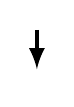
\begin{tikzpicture}[ultra thick]
 \draw [black,   -latex      ] (0,0.5) -- (0,0) node [] {};
\end{tikzpicture}
\end{minipage}

\begin{subfigure}[b]{\linewidth}
\centering
\begin{minipage}{.85\textwidth}
\begin{lstlisting}[mathescape,numbers=left]
int4 mul3(int4 x) { return x * 3; }
kernel map_mul3(global int* in,out, int len) {
  // division into workgroup by chuncks of 1024
  for (int i=get_group_id; i < len/1024;
       i+=get_num_groups) {
    global int* grp_in  = in+(i*1024);
    global int* grp_out = out+(i*1024);
    // division into threads by chunks of 4
    for (int j=get_local_id; j < 1024/4;
         j+=get_local_size) {
      global int* lcl_in  = grp_in+(j*4);
      global int* lcl_out = grp_out+(j*4);
      // vectorization with vector width of 4
      global int4* in_vec4 = (int4*) lcl_in;
      global int4* out_vec4 = (int4*) lcl_out;
      *out_vec4 = mul3(*in_vec4);      
} } }  
\end{lstlisting}
\end{minipage}
\caption{\textbf{OpenCL program} automatically produced by our code generator.}
\label{fig:codeex:ocl}
\end{subfigure}

\caption{Pseudo-code representing a vector scaling program.
The user simply maps the \texttt{mul3} function over the elements of the input array~(\subref{fig:codeex:map}).
This high-level expression is automatically transformed into a low-level expression~(\subref{fig:codeex:impl}) using rewrite rules.
Finally, our code generator turns the low-level expression into an OpenCL program~(\subref{fig:codeex:ocl}).}
\label{fig:codeex}
\end{figure}

We now present the advantages of our approach with a simple vector scaling example shown in Figure~\ref{fig:codeex}.
The user expresses the computation by writing a high-level expression using our \pat{map} algorithmic pattern as shown in Figure~\ref{fig:codeex:map}.
This coding style is similar to functional and dataflow programming.

Our technique first rewrites automatically the user provided high-level expression into something closer to the OpenCL programming model.
This is achieved by applying the rewrite rules presented later in Section~\ref{rules}.
Figure~\ref{fig:codeex:impl} shows one possible derivation of the original high-level map expression where the $\circ$ operator represents function composition, \ie $f \circ g(x) = f(g(x))$.
Starting from the last line, we first split the input into chunks of 1024 elements.
Each chunk is mapped onto a workgroup with the \pat{map-workgroup} low-level pattern (line~2).
Within a workgroup (lines~3--5), we further split the elements into chunks of 4 (line~5), each mapped to a local thread via the \pat{map-local} low-level pattern (line~3).
Each local thread is responsible for processing 4 elements.
Finally, the \pat{vectorize-4} pattern (line~4) implies that the user defined function \texttt{mul3} is vectorized.
The exact meaning of our patterns will be given later in Section~\ref{pattern}.

The last step consists of traversing the low-level expression and generating OpenCL code (see Figure~\ref{fig:codeex:ocl}) for each low-level pattern encountered.
The two map patterns generate the for loops (line~4--5 and~9--10) that iterate over the input array assigning work to the workgroups and local threads.
The information of how many chunks each workgroup and thread processes comes from the corresponding \pat{split}.
In line~16 the vectorized version of the user defined \texttt{mul3} function (defined in line~1) is finally applied to the input array.

To summarize, our approach is able to automatically generate OpenCL code starting from a high-level representation of a program.
This is achieved by automatically lowering the high-level expression into a low-level form suitable for code generation.
The next two sections present our high-level and low-level patterns, the code generation mechanism and the rewrite rules in more details.
\from{PACT end}


\from{PACT begin}
\section{Patterns Design and Implementation (PACT)}
\captionsetup[table]{margin=1.75em}
\begin{table*}[th]
\centering
\rowcolors{2}{oddcolor}{evencolor}
\begin{tabular}{lll}
\toprule
\tabhead{Pattern} & \tabhead{Type} & \tabhead{Description}\\
\midrule
 \pat{id}             & $T[n] \rightarrow T[n]$                                & Identity function.\\
 \pat{map(f)}         & $T[n] \rightarrow U[n], f: T \rightarrow U$            & Apply function $f$ to every element of the input array.\\
 \pat{reduce(f, z)}   & $T[\ ] \rightarrow T[1], f: (T,T) \rightarrow T, z : T$& Apply the reduction function $f$ with initial value z to the input array.\\
 \pat{iterate$^n$(f)} & $T[\ ] \rightarrow T[\ ], f: T[\ ] \rightarrow T[\ ]$  & Iterate the function $f$ over the input $n$ times.\\
 \pat{transpose}      & $T[m][n] \rightarrow T[n][m]$                          & Transpose the 2D input array.\\ 
 \pat{zip(a,b)}       & $a:T[n], b:U[n] \rightarrow \langle T,U \rangle [n]$   & Zip two arrays into an array of pairs.\\
 \pat{innerSplit}$^n$ & $T[\ ]^*[q] \rightarrow T[\ ]^*[m][n], m \cdot n = q$  & Splits the inner most dimension of an array in chunks of size n.\\
 \pat{outerSplit}$^n$ & $T[q][\ ]^* \rightarrow T[m][n][\ ]^*, m \cdot n = q$  & Splits the outer most dimension of an array in chunks of size n.\\
 \pat{innerJoin}$^n$  & $T[\ ]^*[m][n] \rightarrow T[\ ]^*[q], m \cdot n = q$  & Joins the two inner most dimensions of an array.\\
 \pat{outerJoin}$^n$  & $T[m][n][\ ]^* \rightarrow T[q][\ ]^*, m \cdot n = q$  & Joins the two outer most dimensions of an array.\\
 \pat{reorder}        & $T[n] \rightarrow T[n]$                                & Reorder the element of the input array.\\
\bottomrule
\end{tabular}
\caption{High-level algorithmic patterns used by the programmer. $T \rightarrow U$ means the function input type is $T$ and output type $U$. We write $T[n]$ for an array of type $T$ with size $n$ and $[\ ]^*$ denotes an arbitrary number of dimensions in an array.}
\label{tab:hlskel}
\end{table*}
%
\begin{table*}[th]
\centering
\rowcolors{2}{oddcolor}{evencolor}
\setlength{\tabcolsep}{2pt}
\begin{tabular}{lll}
\toprule
\tabhead{Pattern} & \tabhead{Type} & \tabhead{Description}\\
\midrule
 \pat{map-workgroup(f)}    & identical to \pat{map(f)}                     & Each \textbf{workgroup} applies function $f$ on a different element of the input array.\\
 \pat{map-local(f)}        & identical to \pat{map(f)}                     & Each \textbf{local thread} applies function $f$ on a different element of the input array.\\
 \pat{map-warp(f)}         & identical to \pat{map(f)}                     & Each \textbf{warp} applies function $f$ on a different element of the input array.\\
 \pat{map-lane(f)}         & identical to \pat{map(f)}                     & Each \textbf{lane thread} applies function $f$ on a different element of the input array.\\
 \pat{map-seq(f)}          & identical to \pat{map(f)}                     & Apply function $f$ to every element of the input array \textbf{sequentially}.\\
 \pat{reduce-seq(f,z)}     & identical to \pat{reduce(f,z)}                & Apply reduction function $f$ with initial value z to the input \textbf{sequentially}.\\  
 \pat{reorder-stride}$^s$  & identical to \pat{reorder}                    & Access input array with a stride $s$ to maintain \textbf{memory coalescing}.\\
 \pat{asLocal(f)}          & $T[\ ] \rightarrow U[\ ], f: T[\ ] \rightarrow U[\ ]$  & Change the storage location for the results of function $f$ to \textbf{local memory}.\\
 \pat{asGlobal(f)}         & $T[\ ] \rightarrow U[\ ], f: T[\ ] \rightarrow U[\ ]$  & Change the storage location for the results of function $f$ to \textbf{global memory}.\\
 \pat{vect}$^n$\pat{(f)}   & $T[n] \rightarrow U[n], f: T \rightarrow U$   & \textbf{Vectorize} the function $f$ by a factor $n$.\\
\bottomrule
\end{tabular}
\caption{Low-level hardware patterns used for code generation. The hardware paradigm used is highlighted in bold in the description.}
\label{tab:llskel}
\end{table*}

One of the key ideas of this paper is to expose algorithmic choices and hardware-specific program optimizations as patterns that can be automatically derived using a rule rewriting system.
The high-level expressions consist of algorithmic patterns that the programmer is expected to use directly.
The low-level expressions consist of hardware patterns representing hardware specific concepts expressible with the OpenCL programming model.

This section discusses the design of our patterns and how we implement them in our OpenCL code generator.
We define our patterns as functions which are implicitly applied to exactly one input array and produces one output array.
To simplify our implementation we decided to encode all types as arrays with primitives represented with arrays of length 1.
The only exceptions are the user-provided functions such as the \texttt{mul3} function in Figure~\ref{fig:codeex:map} that operates on a primitive type.


\subsection{Algorithmic Patterns}

Table~\ref{tab:hlskel} presents our high-level algorithmic patterns.
These patterns are not tied to any specific hardware feature and are used to define the program at the algorithmic level by the programmer.
The widely known patterns \pat{id}, \pat{map}, and \pat{reduce} have their usual meaning and should be self-explanatory.
 
\paragraph{Iterate}
The \pat{iterate} pattern corresponds to the mathematical definition of iteratively applying a function.
It is defined as: {$f^0 = id$} and {$f^{n+1} = f^n \circ f$}.
In terms of implementation, our code generator emits a for-loop to perform the iteration, and two pointers for input and output.
After each iteration, we swap the pointers, so that the output of the last iteration becomes the input for the next one.
We automatically allocated and calculate memory requirements based on the information from the input and output type.

\paragraph{Transpose, Zip and Split/Join}
These patterns mainly transform the shape of the data and we store this information in the type system.
As a result our code generator does not emit any code.
The \pat{transpose} pattern simply transposes a 2D array while the \pat{zip} pattern fuses two arrays into an array of pairs.
The \pat{split} pattern, which is most often combined with a \pat{join} is similar to the split-join concept from data flow languages such as StreamIt~\cite{thies02streamit}.
\pat{Split} partitions an array into chunks of specific size resulting in an extra dimension.
There exist two variants of split; \pat{innerSplit} and \pat{outerSplit}.
They differ in the dimension used to perform the split; the inner most or outer most respectively.
The corresponding join functions do the opposite of the split functions; they reassemble arrays of arrays by merging dimensions.

\paragraph{Reorder}

The \pat{reorder} pattern allows our system to reorder arbitrarily the elements of an array.
In effect, this function can be used to specify that the ordering of the elements of an array does not matter in a given algorithm.
No code is generated for this pattern since it is always lowered into low-level hardware patterns according to our rewrite rules.



\subsection{Hardware-specific Patterns}

As seen in Section~\ref{gpu}, parallel machines such as GPUs can be quite complex.
In order to achieve the highest performance, programmers often use a set of rules of thumb to drive the optimization of their application for the specific devices.
In fact each hardware vendor provides optimization guides~\cite{nvidia11guide,amd12guide} that extensively cover hardware particularities and how to optimize OpenCL code for them.

In this section, we formalize hardware paradigms by expressing them as patterns.
Table~\ref{tab:llskel} gives an overview of all the hardware-specific patterns we have identified.
These patterns encode the OpenCL programming model.

\paragraph{Parallel Maps}

The different map patterns represent possible ways of mapping computations and exploit parallelism.
For instance, the \pat{map-workgroup(f)} pattern assigns work to workgroups by letting every workgroup apply the function $f$ on a different element of the input array.
Similarly, the other map patterns assign work to local threads, warps, or threads inside a warp (lane threads).
This allows us to map computations to the thread hierarchy of OpenCL as shown in Figure~\ref{fig:map}.
One key finding of our paper is that these map patterns are in effect all we need to express parallelism.

The code generation for all these map patterns is similar, we describe it using \pat{map-workgroup(f)} as example.
A loop is generated, where the iteration variable is determined by the \emph{workgroup-id}, which is provided by OpenCL.
Inside of the loop, a pointer is generated to partition the input array, so that every workgroup processes a different chunk of data.
We use this pointer as the input for the function $f$ being bound to the map.
Similarly, we generate and use a pointer for the output.
After emitting the code for the loop, we continue with the body of the loop by generating the code for the function $f$.
When the generation of the body is finished, an appropriate synchronization mechanism for the given map pattern is added.
For instance after a \pat{map-local} we add a barrier synchronization to synchronize the threads inside of the workgroup.

An interesting aspect of this approach is that we can automatically optimize away some of the synchronization barriers.
On most GPUs, it is possible to avoid synchronization when dealing with threads within the same warp since they are implicitly synchronized (Figure~\ref{fig:map}).
As a result the implementation of \pat{map-lane} does not emit any synchronization.



\paragraph{Sequential Map and Reduce}
The \pat{map-seq(f)} pattern is used to perform a map sequentially within a single thread.
Similarly, \pat{reduce-seq(f, ne)} performs a sequential reduction within a single thread.
In both cases the generated code consists of a simple for loop iterating over the array and calling the function $f$.
In case of the reduction, an accumulator variable is used and initialized with the first element of the input.

\paragraph{Reorder-stride}
This pattern reorders the elements of an array of size $n$ with a stride $s$.
In effect, this generates an output array such that $ out[i] = in[(i / n) + s \cdot (i \mod n)] $.
This hardware pattern is useful to ensure accesses to the device memory stay coalesced when splitting the workload among threads.

Our implementation of this pattern does not produce code directly, but generates instead an index function, which is used when accessing the array.
Therefore, any following read implicitly reorders the array.
While not discussed here, our design allows us to support user-defined index functions.

\paragraph{Local/Global}
The \pat{asLocal(f)} and \pat{asGlobal(f)} patterns are used to determine where the result of function $f$ should be stored.
With these two patterns, we can in effect exploit the memory hierarchy and the local memory.
These patterns act similarly to a typecast and are in fact implemented as such so that no code is emitted.

In our design, every function reads its input and writes its output using pointers provided by the callee function.
As a result, we can simply force a store to local memory by wrapping any function with our \pat{asLocal} pattern.
In the code generator, this will simply change the output pointer of function $f$ to an area in local memory.

\paragraph{Vectorize}
The \pat{vect$^n$(f)} pattern allows us to vectorize a function.
From a semantic point of view it changes the input and output type of function $f$ by replacing any scalar types to vector types.
For instance, in OpenCL an array of \texttt{int} could be transformed into an array of \texttt{int4} as seen in the motivation example (Figure~\ref{fig:codeex}).
In our current implementation, we can vectorize functions containing only simple arithmetic operations, like $+$ or $-$.
In the case of larger functions, we rely on external tools~\cite{garrenberg11vect} for vectorizing more complex functions.


\begin{figure}[t]
\centering
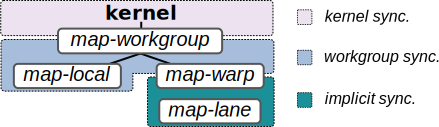
\includegraphics[width=0.8\linewidth]{PACT2014/map}
\caption{Map hierarchy corresponding to the OpenCL hierarchy. Also shown is the type of synchronization available for each stage.}
\label{fig:map}
\end{figure}
\from{PACT end}


\from{PACT begin}
\section{Rewrite Rules (PACT)}

This section introduces our set of rewrite rules that transform high-level expressions written using our algorithmic patterns into semantically equivalent expressions.
One goal of our approach is to keep each rule as simple as possible and only express one fundamental concept at a time.
For instance the vectorization rule, as we will see, is the only place where we express the vectorization concept.
This is different from most prior approaches that would for instance produce a special vectorized version of different algorithmic patterns such as map or reduce.
The superiority of using such an approach lies in the power of composition;
many rules can be applied successively to produce expressions that compose hardware concepts or optimizations and that are correct by construction.

Similarly to our patterns, we distinguish between algorithmic and lowering rules.
Algorithmic rules produces derivations that represent the different algorithmic choices and are shown in Figure~\ref{fig:algo}.
The lowering rules shown in Figure~\ref{fig:low} map expressions to hardware patterns expressible with the OpenCL programming model.
Once the expression is in its lowest form, it is possible to produce OpenCL code easily with our code generator as seen in the previous section.


\paragraph{Syntax and Rule Derivation}
Some rules can only be activated if certain conditions are true.
The syntax $[pre:post]$ represents the pre and post conditions.
The pre condition $pre$ corresponds to the list of conditions that must be true for the rule to be applied.
The post condition $post$ is set for any function bound to the pattern.
The $\overline{\rule[-.3\baselineskip]{0pt}{1.5ex}\hspace{1.5ex}}$, $\wedge$, and $\vee$ corresponds to the logical \emph{not}, \emph{and}, and \emph{or} operators respectively.

We use leftmost derivation when applying the rules, which means that the leftmost non-terminal is always derived first.


\subsection{Algorithmic Rules}

\begin{figure}[t]
\centering
\begin{subfigure}[b]{1\linewidth}
\begin{mdframed}
$$
\begin{array}{lllll}
  f & \rightarrow & f \circ \pat{id} & | & \pat{id} \circ f\\
\end{array}
$$
\end{mdframed}
  \caption{Identity}
  \label{fig:algo:identity}
\end{subfigure}

\vspace{-0.5em}
\begin{subfigure}[b]{1\linewidth}
\begin{mdframed}
$$
\begin{array}{lrl}
  \pat{\textbf{iterate}}^{m+n}\pat{(f)} & \rightarrow & \pat{\textbf{iterate}}^m\pat{(f)} \circ \pat{\textbf{iterate}}^n\pat{(f)}\\
  \end{array}
$$
\end{mdframed}
  \caption{Iterate decomposition}
  \label{fig:algo:iterate}
\end{subfigure}

\vspace{-0.5em}
\begin{subfigure}[b]{1\linewidth}
\begin{mdframed}
$$
\begin{array}{lrl}
  \pat{map(f)} \circ \pat{reorder} & \rightarrow & \pat{reorder} \circ \pat{map(f)}\\
  \pat{reorder} \circ \pat{map(f)} & \rightarrow & \pat{map(f)} \circ \pat{reorder}\\  
\end{array}
$$
\end{mdframed}
  \caption{Reorder commutativity}
  \label{fig:algo:reorder}
\end{subfigure}

\vspace{-0.5em}
\begin{subfigure}[b]{1\linewidth}
\begin{mdframed}
$$
\begin{array}{lrl}
  \pat{map(f)} & \rightarrow & \pat{\textbf{outerJoin}} \circ \pat{map(map(f))}\circ \pat{\textbf{outerSplit}}^n
\end{array}
$$
\end{mdframed}
  \caption{Split-join}
  \label{fig:algo:splitjoin}
\end{subfigure}

\vspace{-0.5em}
\begin{subfigure}[b]{1\linewidth}
\begin{mdframed}
$$
\begin{array}{lrl}
\multicolumn{3}{l}{\pat{part-red(f,z)} \rightarrow} \\
  & & \pat{reduce(f,z)}\\                                                      
  &| & \pat{part-red(f,z)} \circ \pat{reorder}\\    
  &| & \pat{\textbf{outerJoin}} \circ \pat{map(part-red(f,z))} \circ \pat{\textbf{outerSplit}}^n\\
  &| & \pat{\textbf{iterate}}^{n}\pat{(part-red(f,z))}\\
\end{array}
$$
$$
\begin{array}{lrl}
  \pat{reduce(f,z)} & \rightarrow & \pat{reduce(f,z)} \circ \pat{part-red(f,z)}\\
  & | & \pat{\textbf{iterate}}^{\infty}\pat{(part-red(f,z))}\\

\end{array}
$$
\end{mdframed}
  \caption{Reduction}
  \label{fig:algo:red}
\end{subfigure}

\vspace{-0.5em}
\begin{subfigure}[b]{1\linewidth}
\begin{mdframed}
$$
\begin{array}{lrll}
\multicolumn{2}{l}{\pat{map(f)} \rightarrow} \\
 {\ }   & \pat{\textbf{innerJoin}} \circ \pat{map(\textbf{vect}}^n\pat{(f))} \circ \pat{\textbf{innerSplit}}^n & [\hspace{.2em}\overline{vec}:vec\hspace{.2em}]
\end{array}
$$
\end{mdframed}
  \caption{Vectorization}
   \label{fig:algo:vect}
\end{subfigure}

\vspace{-0.5em}
\begin{subfigure}[b]{1\linewidth}
\begin{mdframed}
$$
\begin{array}{lrl}
f \circ \pat{id}\ |\ \pat{id} \circ f & \rightarrow & f\\
\pat{\textbf{outerSplit}}^n \circ \pat{\textbf{outerJoin}}^n & \rightarrow & \pat{id}\\
\pat{\textbf{innerSplit}}^n \circ \pat{\textbf{innerJoin}}^n & \rightarrow & \pat{id}\\
\end{array}
$$
\end{mdframed}
  \caption{Simplification rules}
   \label{fig:algo:simpl}
\end{subfigure}

\vspace{-0.5em}
\begin{subfigure}[b]{1\linewidth}
\begin{mdframed}
$$
\begin{array}{lll}
\pat{map(f)} \circ \pat{map(g)}                                & \rightarrow & map(f \circ g)\\
\pat{\textbf{reduce-seq}(f,z)} \circ \pat{\textbf{map-seq}(g)} & \rightarrow & \\
{\ \ } \pat{\textbf{reduce-seq}}(\lambda\ acc,x: f(acc,g(x)), z)\\
\end{array}
$$
\end{mdframed}
  \caption{Fusion rules}
   \label{fig:algo:fusion}
\end{subfigure}
\vspace{-2em}
\caption{Algorithmic rules. Bold patterns are known to the code generator.}
\label{fig:algo}
\end{figure}

\begin{figure}[t]
\centering

\begin{subfigure}[b]{1\linewidth}
\begin{mdframed}
$$
\begin{array}{lll}
\multicolumn{3}{l}{\pat{map(f)} \rightarrow} \\
       & \pat{\textbf{map-workgroup}(f)} & [\hspace{.2em}\overline{mwg}:mwg\hspace{.2em}]\\
{\ } | & \pat{\textbf{map-local}(f)    } & [\hspace{.2em}\overline{mlc}\hspace{.7em} \wedge mwg\wedge\overline{mwp}:mlc\hspace{.2em}]\\
{\ } | & \pat{\textbf{map-warp}(f)     } & [\hspace{.2em}\overline{mwp}\hspace{.2em} \wedge mwg\wedge\overline{mlc}:mwp\hspace{.2em}]\\
{\ } | & \pat{\textbf{map-lane}(f)     } & [\hspace{.2em}\overline{mln}\hspace{.5em} \wedge mwp:mln\hspace{.2em}]\\
{\ } | & \pat{\textbf{map-seq}(f)   } & [\hspace{.2em}\overline{msr}\hspace{.5em} \wedge (mlc\vee mln):msr\hspace{.2em}]\\          
\end{array}
$$
\end{mdframed}
  \caption{Map}
  \label{fig:low:map}
\end{subfigure}

\vspace{-0.5em}
\begin{subfigure}[b]{1\linewidth}
\begin{mdframed}
$$
\begin{array}{llll}
  \pat{reduce(f,z)} & \rightarrow & \pat{\textbf{reduce-seq}(f,z)} & [\hspace{.2em}mlc\vee mln:\ \hspace{.2em}]\\   
\end{array}
$$
\end{mdframed}
  \caption{Reduction}
  \label{fig:low:red}
\end{subfigure}

\vspace{-0.5em}
\begin{subfigure}[b]{1\linewidth}
\begin{mdframed}
$$
\begin{array}{lrl}
  \pat{\textbf{map-local}(f)} & \rightarrow & \pat{\textbf{asGlobal}(map-local(f))}\\  
  \pat{\textbf{map-local}(f)} & \rightarrow & \pat{\textbf{asLocal}(map-local(f))}\\  
\end{array}
$$
\end{mdframed}
  \caption{Local/Global memory}
  \label{fig:low:mem}
\end{subfigure}

\vspace{-0.5em}
\begin{subfigure}[b]{1\linewidth}
\begin{mdframed}
$$
\begin{array}{lllll}
  \pat{reorder}  & \rightarrow & \pat{\textbf{reorder-stride}}^s & | & \pat{id}
\end{array}
$$
\end{mdframed}
  \caption{Stride accesses or normal accesses}
  \label{fig:low:stride}
\end{subfigure}
\vspace{-2em}
\caption{Lowering rules. Bold patterns are known to the code generator.}
\label{fig:low}
\end{figure}



The first three rules (see Figure~\ref{fig:algo:identity},~\ref{fig:algo:iterate} and~\ref{fig:algo:reorder}) express the properties of the identity, iterate and reorder pattern.


\paragraph{Split-join}
The split-join rule in Figure~\ref{fig:algo:splitjoin} partitions a map into two maps.
This allows us to nest maps in each other and, thus, \emph{map} the computation to the thread hierarchy of the OpenCL programming model such as \pat{map-workgroup(map-local(f))} as seen in our motivation example (Figure~\ref{fig:codeex}).


\paragraph{Reduction}
The reduction (and associated partial reduction) in Figure~\ref{fig:algo:red} is currently our most complex rule but also the most powerful one.
It allows us to express the reduction function as a composition of other primitive functions, which is a fundamental aspect of our work.
From the algorithmic point of view we first define a partial reduction pattern \pat{part-red}.
This partial reduction reduces an array of $n$ elements to an array of $m$ elements where $1 \leq m < n$.
The reduction can be derived in a partial reduction combined with a full reduction which ensures we end up with one unique element.
Another possible derivation consists in iterating a partial reduction until a full reduction is achieved (this is what $\infty$ represents).

Note that our definition of \pat{reduce} remains correct since the result of a partial reduction is always composed with the reduction to ensure we end up with one unique element.

\paragraph{Partial Reduction}
The first possible derivation for partial reduction, in Figure~\ref{fig:algo:red}, leads to the full reduction which means $m=1$.
The next possible derivation expresses the fact that it is possible to reorder the elements to be reduced, expressing the commutativity property of our definition of reduction.
The fourth derivation is actually the only place where parallelism is expressed in the definition of our reduction pattern.
This rule expressed the fact that it is valid to partition the input elements first and then reduce them independently.
Finally, the last possible derivation expresses the notion that it is possible to perform a partial reduction with an iterative process by repetitively applying the same partial reduction function.
This concept is very important when considering how the reduction function is typically implemented on a GPU (iteratively reducing within a workgroup using the local memory).

\paragraph{Vectorization}
Figure~\ref{fig:algo:vect} shows the vectorization rule.
Vectorization is achieved by using the \pat{innerSplit} and corresponding \pat{innerJoin} which split the data on the innermost dimension only.
The rule \emph{pre} and \emph{post} conditions ensure that vectorization is applied only once in any expression derived from $f$.
Another set of rules, not shown here for space reason, are used to propagate the $vect^n$ function recursively within $f$.

\paragraph{Simplification Rules}
Figure~\ref{fig:algo:simpl} shows our simplification rules.
They express the property of the $id$ function and the removal of consecutive splits and joins.

\paragraph{Fusion Rules}
Finally, our fusion rules are shown in Figure~\ref{fig:algo:fusion}.
The first rule allows us to fuse the functions applied by two consecutive maps.
The second rule fuses the map-reduce pattern by creating a lambda function that is the results of merging function $f$ and $g$ from the original reduction and map respectively.
Note that this rule only applies to the sequential version since this is the only implementation that does not require the associativity property required by the more generic $\pat{reduce}$ pattern.
When generating code, these rules in effect allow us to fuse the implementation of the different functions and avoid having to store temporary results.





\subsection{Lowering Rules}

Our lowering rules are shown in Figure~\ref{fig:low}.
The purpose of these rules is to lower high-level expressions to low-level expressions, which consist only of hardware patterns for which we can generate code.
These hardware patterns are highlighted in bold in Figure~\ref{fig:algo} and~\ref{fig:low}.

\paragraph{Maps}
The rule shown in Figure~\ref{fig:low:map} is used to produce the different low-level \pat{maps}.
The \emph{pre} and \emph{post} conditions reflect the hierarchy presented in Figure~\ref{fig:map} corresponding to the OpenCL programming model.
For instance for \pat{map-workgroup}, we have the pre condition that we must not be within a \pat{map-workgroup} ($\overline{mwg}$) already.

\paragraph{Reduction}
There is only one lowering rule for reduction (Figure~\ref{fig:low:red}), which expresses the fact that the only OpenCL implementation known to the code generator is a sequential reduction.
The reduction pattern is defined at a higher level by composing other algorithmic patterns.
To the best of our knowledge, all other existing high performance compilers treat the reduction directly as an irreducible primitive operation.
The power of our approach is that the code generator implementation only needs to know about the simple sequential reduction.
As a result, it is possible to explore different implementation for the reduction automatically by simply applying different rules.

\paragraph{Local/Global}
Figure~\ref{fig:low:mem} shows the two rules that allow us to make use of the GPU local memory.
These rules express the fact that the result of a \pat{map-local} can always be stored in local memory or back in global memory.
This holds because a \pat{map-local} always exists within a \pat{map-workgroup} where the local memory is defined.
These rules allow us to determine how the data is mapped to the GPU memory hierarchy.

\paragraph{Reorder}
Finally, Figure~\ref{fig:low:stride} presents the rule that reorders elements of an array.
In our current implementation, we support two types of reordering:
no reordering, represented by the \pat{id} function, and \pat{reorder-stride} which reorders elements with a certain stride $s$.
As described earlier, the major use case for the stride reorder is to enable coalesced memory accesses.


\subsection{Automatic Rewriting Strategy}
\label{sec:search}

The rules presented in this section define a search space of possible implementations.
In order to find the best possible low-level expression for a given target device, we have developed a simple automatic search strategy based loosely on Bandit-based optimization~\cite{demesmay09bandit}.
Note that our current search strategy is just designed to prove that it is possible to find good implementations.
We envision replacing this exploration strategy in the future by using machine-learning techniques to avoid having to search the space.
However, this is orthogonal to the work presented in this paper.

Our search strategy starts with the high-level expression and determines all the valid rules that can be applied at this stage.
We use a Monte-Carlo method for evaluating the potential impact of each rule by randomly walking down the search tree.
The rule that will lead to the best performance following the Monte-Carlo descent is chosen and applied to the expression.
This process is repeated until we reach a terminal expression.
Note that in addition to selecting the rules, we also search at the same time for the parameters controlling our patterns such as the vector size for the $\pat{vect}^n$ pattern.
Using this simple strategy, we found that less than a thousand expressions were evaluated to reach a solution in most cases.


\subsection{Summary}

The power of our approach lies in the composition of our rules that produce complex expressions.
Looking back at our motivation example in Figure~\ref{fig:codeex}, we can see how a simple algorithmic pattern such as \pat{map} can be effectively derived into a low-level expression by applying our rules.
This expression matches various hardware concepts expressible with the OpenCL programming model such as mapping computation and data to the GPU thread and memory hierarchy respectively and vectorization.
Using these rules and our automatic search technique we now have a powerful mechanism to explore the space of possible program implementations.
\from{PACT end}


\from{PACT begin}
\section{Implementation Details (PACT)}

Our system is implemented in C++11, using the template system and support for lambda functions. 
When generating code for a given low-level expression, two basic steps are performed.
First, we use the Clang/LLVM compiler library to parse the expression and produce an abstract syntax tree for it.
Second, we traverse the tree and emit code for every function call representing one of our low-level hardware patterns.

As part of the first step, we have developed a type system which plays a dual role.
Firstly, it prevents the user, or a rewrite rule, to produce an expression that is not correct.
Secondly, the type system encodes informations that are necessary for code generation, such as memory address space and array size information, which are used to allocate memory.

The design of our code generator is straightforward since no optimization decisions are made at this stage.
We avoid performing complex analysis of the code which makes our design very different compared to traditional optimizing compilers.

\from{PACT end}

